\documentclass{article}

\usepackage{graphicx}
\usepackage{textcomp}
\usepackage{xcolor}
\usepackage{tikz}
\usepackage{pgfplots}
\usepackage{filecontents}

\begin{document}

\author{
  Blake, Christopher\\
  \texttt{chriswblake@gmail.com}
}

\title{Sample drawings}
\maketitle

%Example distribution chart with data
Distribution Chart with Data

\newcommand{\bin}[5]{
    %Bounding box
    \draw [gray!25] (0,0) rectangle (10,1);

    %Low and High
    \draw [gray] (#1, 0.8) -- (#1, 0.05); \node [black] at (#1, 0.9) {$Low$};
    \draw [gray] (#2, 0.8) -- (#2, 0.05); \node [black] at (#2, 0.9) {$High$};

    %Distribution curve
    \draw [gray, thick, dashed] plot [smooth] coordinates {
        (#3, 0.3) (#3+1, 0.4)
        (#4, 0.8)
        (#5-1, 0.4) (#5, 0.3)};

    %-Nsigma, Average, +NSigma
    \draw [gray] (#3, 0.2) -- (#3, 0.4); \node [black] at (#3, 0.1) {$-N\sigma$};
    \draw [gray] (#4, 0.2) -- (#4, 0.95); \node [black] at (#4, 0.1) {$\mu$};
    \draw [gray] (#5, 0.2) -- (#5, 0.4); \node [black] at (#5, 0.1) {$+N\sigma$};
}
\begin{tikzpicture} [yscale=1.5]
    %Low,High,-NSigma,Avg,+NSigma
    \bin{1.0}{9.0}{0.5}{5.0}{9.5}
    
    %Data points
    \foreach \Point in {
        (2.0, 0.4), (4.0, 0.4), 
        (5.0, 0.4),
        (6.0, 0.4), (8.0, 0.4)}
        {\node [black] at \Point {\textbullet};}
\end{tikzpicture}


%Histogram


%------------------------
\section{Loading data}
    Examples Gallery: http://pgfplots.sourceforge.net/gallery.html
    
    %--------------------------
    \subsection{Cubic spline}
    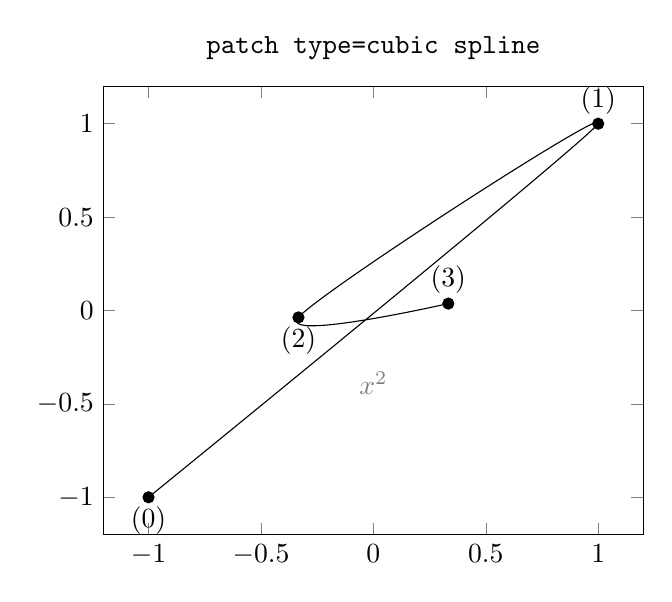
\begin{tikzpicture}
        \begin{axis}[nodes near coords={(\coordindex)},
            title={\texttt{patch type=cubic spline}}]
            \addplot[
                mark=*,
                %patch,
                %mesh,
                smooth
                ]
            coordinates {
                % left, right, left middle, right middle
                (-1,-1) 
                (1,1)  
                (-1/3,{(-1/3)^3})
                (1/3,{(1/3)^3})
            };
            \node [above,gray] at (0,-0.5) {$x^2$};
        \end{axis}
        
    \end{tikzpicture}

    %--------------------------
    \subsection{Histogram from loaded file}
    \begin{tikzpicture}
    \begin{axis}[
      ybar interval,
      width=0.5\columnwidth,
      xtick=,% reset from ybar interval
      xticklabel=
        {$[\pgfmathprintnumber\tick,%
           \pgfmathprintnumber\nexttick)$}
    ]

    \addplot+[hist={data=x}]
        file {plotdata/pgfplots.randn.dat};
        
    \end{axis}
    \end{tikzpicture}

    %---------------------------
    \subsection{Multiple series from inline data set}
    \begin{filecontents}{pistonkinetics.dat}
        eang    disppos dispvel dispacc 
        0.0000  50.0000 0.0000  -32.8125
        1.0000  49.9950 -0.5726 -32.8043
        2.0000  49.9800 -1.1450 -32.7796
        3.0000  49.9550 -1.7168 -32.7386
        4.0000  49.9201 -2.2877 -32.6811
        5.0000  49.8752 -2.8575 -32.6073
        6.0000  49.8204 -3.4258 -32.5172
        7.0000  49.7556 -3.9924 -32.4108
        8.0000  49.6810 -4.5571 -32.2882
        9.0000  49.5966 -5.1194 -32.1495
        10.0000 49.5023 -5.6792 -31.9948  
        11.0000 49.3983 -6.2361 -31.8241
        12.0000 49.2847 -6.7900 -31.6376
        13.0000 49.1613 -7.3404 -31.4354
        14.0000 49.0284 -7.8872 -31.2176
        15.0000 48.8860 -8.4300 -30.9844
        16.0000 48.7342 -8.9687 -30.7358
        17.0000 48.5730 -9.5028 -30.4721
        \end{filecontents}

    \pgfplotstableread{pistonkinetics.dat}{\pistonkinetics}
    \begin{tikzpicture}[scale=1]
    \begin{axis}[minor tick num=1,
    xlabel=Degrees]
    \addplot [black,very thick] table [x={eang}, y={disppos}] {\pistonkinetics};
    \addplot [dashed,red,very thick] table [x={eang}, y={dispvel}] {\pistonkinetics};
    \addplot [dashed,blue,very thick] table [x={eang}, y={dispacc}] {\pistonkinetics};
    \end{axis}
    \end{tikzpicture}











4 lines to make a box

\begin{tikzpicture}
    \draw (0,0) -- (4,0) -- (4,4) -- (0,4) -- cycle;
\end{tikzpicture}


Rectangle to make a box

\begin{tikzpicture}
    \draw (0,0) rectangle (4,4);
\end{tikzpicture}


Parabola

\begin{tikzpicture}
    \draw (0,0) parabola (4,4);
\end{tikzpicture}


Spline inside cirle

\begin{tikzpicture}[scale=1.1]
    \draw (0,0) .. controls (0,4) and (4,0) .. (4,4);
    \draw[red,thick,dashed] (2,2) circle (3cm);
\end{tikzpicture}


Ellipse and Arc

\begin{tikzpicture}
    \draw (2,2) ellipse (3cm and 1cm);
    \draw (8,0) arc (0:75:3cm);
\end{tikzpicture}


Grid

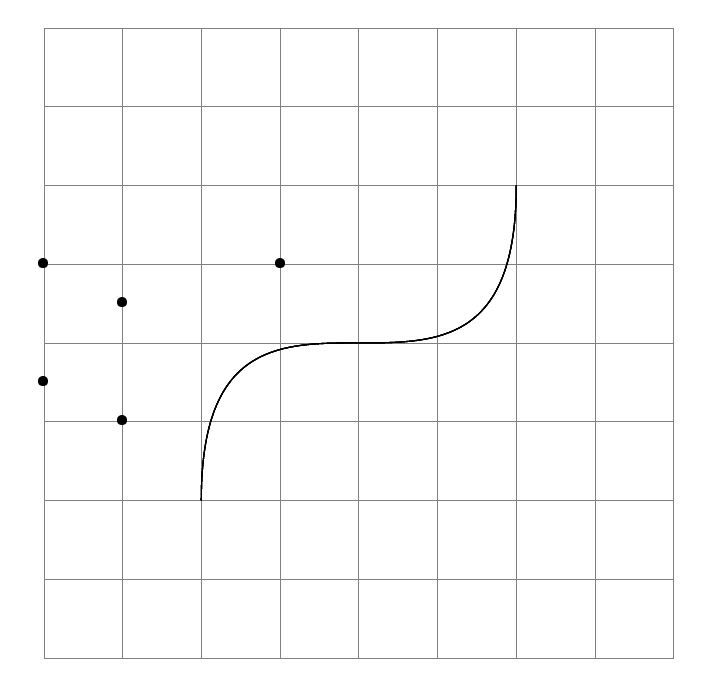
\begin{tikzpicture} [stuff/.style={ draw, circle, fill} ]
    \draw[step=1cm,gray,very thin] (-2,-2) grid (6,6);

    \foreach \Point in {(-2,1.5), (-1,1), (-2,3), (-1,2.5), (1,3)}{
        \node [black] at \Point {\textbullet};
    
    \draw (0,0) .. controls (0,4) and (4,0) .. (4,4);
    % \foreach \Point2 in {(-1,1.5), (-0,1), (-1,3), (-0,2.5), (2,3)}{
    % \node [blue] at \Point2 {$\circ$};
}
\end{tikzpicture}


Grid, trimmed

\begin{tikzpicture}
    \draw[step=1cm,gray,very thin] (-1.9,-1.9) grid (5.9,5.9);
\end{tikzpicture}

\end{document}